\frameT{Relations and Orderings}{
  \begin{block}{Binary Relations}
		Let $O$ be a set of elements. A \tit{binary relation} $\preceq$ over $O$ is a
		collection of ordered pairs of elements in $O$; that is,
		\begin{center}
			$\preceq \; \subseteq O \times O$.
		\end{center}
  \end{block}

	Properties of binary relations:
	\begin{enumerate}
		\item Reflexivity: $\forall o \in O$, $o\preceq o$.
		\item Irreflexivity: $\forall o \in O$, $o\not\preceq o$.
		\item Totality: $\forall o_1,o_2$, $o_1\preceq o_2$ or $o_2\preceq o_1$.
		\item Transitivity: $\forall o_1,o_2,o_3$, if $o_1\preceq o_2$ and $o_2\preceq o_3$, then $o_1\preceq o_3$.
		\item Symmetricity: $\forall o_1,o_2$, if $o_1\preceq o_2$, then $o_2\preceq o_1$.
		%\item Asymmetricity: $\forall o_1,o_2$, if $o_1\preceq o_2$, then $o_2\not\preceq o_1$.
		\item Antisymmetricity: $\forall o_1,o_2$, if $o_1\preceq o_2$ and $o_2\preceq o_1$, then $o_1=o_2$.
	\end{enumerate}
}

\frameT{Relations and Orderings}{
  \begin{block}{Binary Relations}
		%A binary relation $\preceq$ over $O$ 
		$\preceq$
		is a \tit{partial preorder} if it is reflexive and
		transitive, a \tit{total preorder} if it is a partial preorder and total, 
		a \tit{partial order} if it is a partial preorder and antisymmetric, and 
		a \tit{total order} if it is a partial order and total.
  \end{block}

	\vspace{-0.3cm}

	\begin{figure}[ht]
	   \small
	  \centering
    \begin{subfigure}[b]{0.45\textwidth}
	  	\centering
		  \begin{tikzpicture}[->,>=stealth',node distance=1.5cm,main node/.style={circle,draw,font=\small}]
		    \node[main node] (1) {$o_1$};
				\node[main node] (2) [below left of=1] {$o_2$};
		  	\node[main node] (3) [below right of=1] {$o_3$};
		  	\node[main node] (4) [below right of=2] {$o_4$};
		
		    \path[every node/.style={font=\sffamily\small}]
		      (4) edge (2)
		      (4) edge (3)
		      (2) edge (1)
		      (3) edge (1)
		      (4) edge (1)
					(1) edge [loop above] (1)
					(2) edge [loop left] (2)
					(3) edge [loop right] (3)
					(4) edge [loop below] (4);
		  \end{tikzpicture}
      \caption{partial (pre)order}
    \end{subfigure}
    \begin{subfigure}[b]{0.45\textwidth}
	  	\centering
		  \begin{tikzpicture}[->,>=stealth',node distance=1cm,main node/.style={circle,draw,font=\small}]
		    \node[main node] (1) {$o_1$};
				\node[main node] (2) [below of=1] {$o_2$};
		  	\node[main node] (3) [below of=2] {$o_3$};
		  	\node[main node] (4) [below of=3] {$o_4$};
		
		    \path[every node/.style={font=\sffamily\small}]
		      (4) edge (3)
		      (4) edge [bend left] (2)
		      (4) edge [bend left] (1)
		      (3) edge (2)
		      (3) edge [bend left] (1)
		      (2) edge (1)
					(1) edge [loop right] (1)
					(2) edge [loop right] (2)
					(3) edge [loop right] (3)
					(4) edge [loop right] (4);
		  \end{tikzpicture}
      \caption{total (pre)order}
    \end{subfigure}
	\end{figure}
}

\frameT{Relations and Orderings}{
  \begin{block}{Binary Relations}
		%A binary relation $\preceq$ over $O$ 
		$\preceq$
		is a \tit{partial preorder} if it is reflexive and
		transitive, a \tit{total preorder} if it is a partial preorder and total, 
		a \tit{partial order} if it is a partial preorder and antisymmetric, and 
		a \tit{total order} if it is a partial order and total.
  \end{block}

	\vspace{-0.3cm}

	\begin{figure}[ht]
	   \small
	  \centering
    \begin{subfigure}[b]{0.45\textwidth}
	  	\centering
		  \begin{tikzpicture}[->,>=stealth',node distance=1.5cm,main node/.style={circle,draw,font=\small}]
		    \node[main node,inner sep=1.2pt] (1)                    {$o_{1,5}$};
				\node[main node,inner sep=1.2pt] (2) [below left of=1]  {$o_{2,6}$};
		  	\node[main node,inner sep=1.2pt] (3) [below right of=1] {$o_{3,7}$};
		  	\node[main node,inner sep=1.2pt] (4) [below right of=2] {$o_{4,8}$};
		
		    \path[every node/.style={font=\sffamily\small}]
		      (4) edge (2)
		      (4) edge (3)
		      (2) edge (1)
		      (3) edge (1)
		      (4) edge (1)
					(1) edge [loop above] (1)
					(2) edge [loop left] (2)
					(3) edge [loop right] (3)
					(4) edge [loop below] (4);
		  \end{tikzpicture}
      \caption{partial preorder}
    \end{subfigure}
    \begin{subfigure}[b]{0.45\textwidth}
	  	\centering
		  \begin{tikzpicture}[->,>=stealth',node distance=1cm,main node/.style={circle,draw,font=\small}]
		    \node[main node,inner sep=1.2pt] (1)              {$o_{1,5}$};
				\node[main node,inner sep=1.2pt] (2) [below of=1] {$o_{2,6}$};
		  	\node[main node,inner sep=1.2pt] (3) [below of=2] {$o_{3,7}$};
		  	\node[main node,inner sep=1.2pt] (4) [below of=3] {$o_{4,8}$};
		
		    \path[every node/.style={font=\sffamily\small}]
		      (4) edge (3)
		      (4) edge [bend left] (2)
		      (4) edge [bend left] (1)
		      (3) edge (2)
		      (3) edge [bend left] (1)
		      (2) edge (1)
					(1) edge [loop right] (1)
					(2) edge [loop right] (2)
					(3) edge [loop right] (3)
					(4) edge [loop right] (4);
		  \end{tikzpicture}
      \caption{total preorder}
    \end{subfigure}
	\end{figure}
}

\frameT{Relations and Orderings}{
  \begin{block}{Binary Relations}
		Let $\preceq$ be a preference relation that is a partial preorder over $O$.
		We say that $o_2$ is \tit{weakly preferred} to $o_1$ if $o_1 \preceq o_2$,
		that $o_2$ is \tit{strictly preferred} ($\prec$) to $o_1$ if $o_1 \preceq o_2$ and
		$o_2 \not \preceq o_1$, that $o_1$ is \tit{indifferent} ($\approx$) from $o_2$ 
		if $o_1 \preceq o_2$ and $o_2 \preceq o_1$, and 
		that $o_1$ is \tit{incomparable} ($\sim$) with $o_2$ if 
		$o_1 \not \preceq o_2$ and $o_2 \not \preceq o_1$.
  \end{block}

	\vspace{-0.3cm}

	\begin{figure}[ht]
	   \small
	  \centering
    \begin{subfigure}[b]{0.45\textwidth}
	  	\centering
		  \begin{tikzpicture}[->,>=stealth',node distance=1.5cm,main node/.style={circle,draw,font=\small}]
		    \node[main node,inner sep=1.2pt] (1)                    {$o_{1,5}$};
				\node[main node,inner sep=1.2pt] (2) [below left of=1]  {$o_{2,6}$};
		  	\node[main node,inner sep=1.2pt] (3) [below right of=1] {$o_{3,7}$};
		  	\node[main node,inner sep=1.2pt] (4) [below right of=2] {$o_{4,8}$};
		
		    \path[every node/.style={font=\sffamily\small}]
		      (4) edge (2)
		      (4) edge (3)
		      (2) edge (1)
		      (3) edge (1)
		      (4) edge (1)
					(1) edge [loop above] (1)
					(2) edge [loop left] (2)
					(3) edge [loop right] (3)
					(4) edge [loop below] (4);
		  \end{tikzpicture}
			\vspace{-0.3cm}
      \caption{partial preorder}
    \end{subfigure}
    \begin{subfigure}[b]{0.45\textwidth}
	  	\centering
			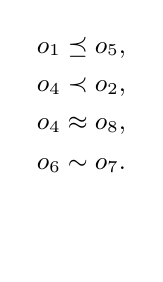
\begin{tikzpicture}[->,>=stealth,node distance=0.5cm,main node/.style={rectangle,font=\small}]
		    \node[main node] (1)              {$o_1 \preceq o_5$,};
		    \node[main node] (2) [below of=1] {$o_4 \prec o_2$,};
		    \node[main node] (3) [below of=2] {$o_4 \approx o_8$,};
		    \node[main node] (4) [below of=3] {$o_6 \sim o_7$.};
		    \node[main node] (5) [below of=4] {};
		    \node[main node] (6) [below of=5] {};
		  \end{tikzpicture}
			\vspace{-0.3cm}
      \caption{preferences}
    \end{subfigure}
	\end{figure}
}

\frameT{Relations and Orderings}{
  \begin{block}{Binary Relations}
		Let $\preceq$ be a preference relation that is a partial preorder over $O$.
		We say that $o_2$ is \tit{weakly preferred} to $o_1$ if $o_1 \preceq o_2$,
		that $o_2$ is \tit{strictly preferred} ($\prec$) to $o_1$ if $o_1 \preceq o_2$ and
		$o_2 \not \preceq o_1$, that $o_1$ is \tit{indifferent} ($\approx$) from $o_2$ 
		if $o_1 \preceq o_2$ and $o_2 \preceq o_1$, and 
		that $o_1$ is \tit{incomparable} ($\sim$) with $o_2$ if 
		$o_1 \not \preceq o_2$ and $o_2 \not \preceq o_1$.
  \end{block}

	\vspace{-0.22cm}

	\begin{figure}[ht]
	   \small
	  \centering
    \begin{subfigure}[b]{0.45\textwidth}
	  	\centering
		  \begin{tikzpicture}[->,>=stealth',node distance=1cm,main node/.style={circle,draw,font=\small}]
		    \node[main node,inner sep=1.2pt] (1)              {$o_{1,5}$};
				\node[main node,inner sep=1.2pt] (2) [below of=1] {$o_{2,6}$};
		  	\node[main node,inner sep=1.2pt] (3) [below of=2] {$o_{3,7}$};
		  	\node[main node,inner sep=1.2pt] (4) [below of=3] {$o_{4,8}$};
		
		    \path[every node/.style={font=\sffamily\small}]
		      (4) edge (3)
		      (4) edge [bend left] (2)
		      (4) edge [bend left] (1)
		      (3) edge (2)
		      (3) edge [bend left] (1)
		      (2) edge (1)
					(1) edge [loop right] (1)
					(2) edge [loop right] (2)
					(3) edge [loop right] (3)
					(4) edge [loop right] (4);
		  \end{tikzpicture}
      \caption{total preorder}
    \end{subfigure}
    \begin{subfigure}[b]{0.45\textwidth}
	  	\centering
			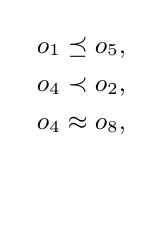
\begin{tikzpicture}[->,>=stealth,node distance=0.5cm,main node/.style={rectangle,font=\small}]
		    \node[main node] (1)              {$o_1 \preceq o_5$,};
		    \node[main node] (2) [below of=1] {$o_4 \prec o_2$,};
		    \node[main node] (3) [below of=2] {$o_4 \approx o_8$,};
		    \node[main node] (4) [below of=3] {};
		    \node[main node] (5) [below of=4] {};
		  \end{tikzpicture}
			\vspace{-0.3cm}
      \caption{preferences}
    \end{subfigure}
	\end{figure}
}

\frameT{Combinatorial Domains}
{
	\begin{block}{Combinatorial Domains}
	  Let $V$ be a finite set of variables $\{X_1,\ldots,X_p\}$,
	  $D$ a set of finite domains $\{\Dom(X_1),\ldots,\Dom(X_p)\}$ for each
	  variable $X_i$.
	  A \tit{combinatorial domain} $\CD(V)$ is a set of \tit{outcomes}
		described by combinations of values from $\Dom(X_i)$:
	  \begin{center}
	    $\CD(V) = \prod_{X_i \in V} \Dom(X_i)$.
	  \end{center}
	\end{block}
}

\frameT{Combinatorial Domains: Example}{
	Domain of cars over set $V$ of $p$ binary variables:
	\begin{enumerate}
		\item \tbf{BodyType}: \{mvan, sedan\}.
		\item \tbf{Capacity}: \{5, 7m\}.
		\item \tbf{Color}: \{blue, grey\}.
		\item[\vdots]
	\end{enumerate}

	\begin{center}
			$\CD(V) = 
				\underbrace{\{\langle\text{sedan, 4, blue, }\ldots\rangle, 
				\langle\text{mvan, 6m, grey, }\ldots\rangle, \ldots\}}_{\text{\large $2^p$ outcomes, too many!}}$.
	\end{center}

%	\begin{center}
%		\begin{align*} 
%			\CD(V) = \{&<\text{sedan, 4, blue, }\ldots>, \\
%								 &<\text{mvan, 6m, grey, }\ldots>, \\
%								 &\ldots\}.
%		\end{align*}
%	\end{center}
}

\frameT{Computational Complexity}{
	\begin{enumerate}
		\item P (NP): decision problems solvable by a deterministic (nondeterministic, resp.) 
					TM in poly time in the size of the input.
		\begin{itemize}
			\item We typically believe that $P \subset \NP$.
		\end{itemize}
		\item coNP: problems whose complements are in NP.
		\item $\deltap{2}$: $P^\NP$.
		\item $\sigmap{2}$: $\NP^\NP$.
		\item PSPACE: decision problems solvable by a
					TM in poly space in the size of the input.
		\item A decision problem $L$ is $C$-hard if $L' \leq_p L$ for every $L'$ in class $C$.
		\item A decision problem $L$ is $C$-complete if $L$ is in class $C$ and
					$L$ is $C$-hard.
	\end{enumerate}
}

\frameT{Computational Complexity}{
	\begin{figure}[ht!]
	  \centering
	    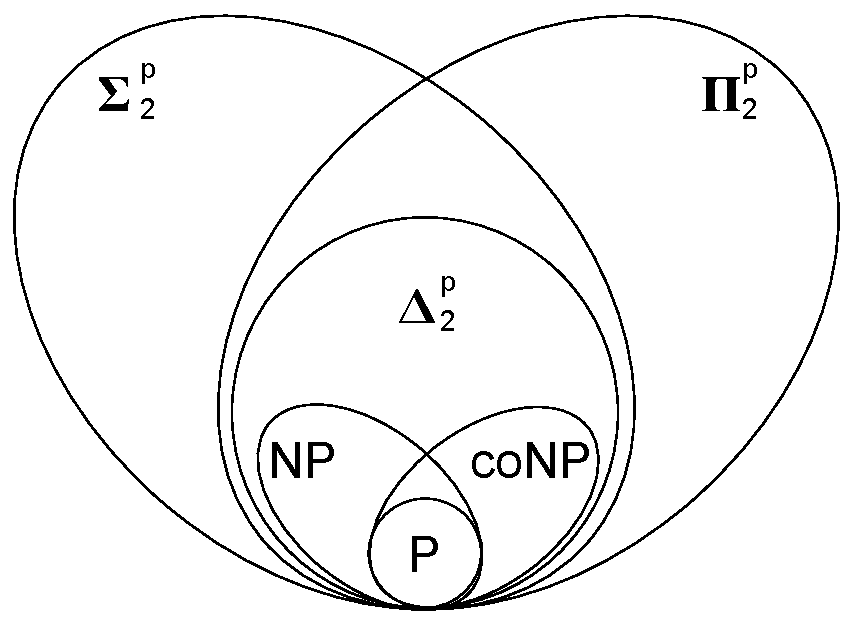
\includegraphics[width=0.65\textwidth]{figs/Preliminary/comp_diagram.pdf}
	  \caption{Computational complexity diagram}
	\end{figure}
}

\frameT{Combinatorial Domains: Example}{
	Domain of cars (cf. the Car Evaluation Dataset\footnotemark)
	\begin{enumerate}
		\item \tbf{BodyType}: \{mvan, sedan, sport, suv\}.
		\item \tbf{Capacity}: \{2, 5, 7m\}.
		\item \tbf{Color}: \{black, blue, grey, red, white\}.
		\item \tbf{LuggageSize}: \{big, med, small\}.
		\item \tbf{Make}: \{bmw, ford, honda, and vw\}.
		\item \tbf{Price}: \{low, med, high, vhigh\}.
		\item \tbf{Safety}: \{low, med, high\}.
	\end{enumerate}
	
	\footnotetext{\tiny \url{http://www.cs.uky.edu/~liu/preflearnlib.php}, slightly
		adapted in the talk.}
}

\frameT{Qualitative Preferences}{
	Individual:
	\begin{figure}[ht!]
	  \centering
	    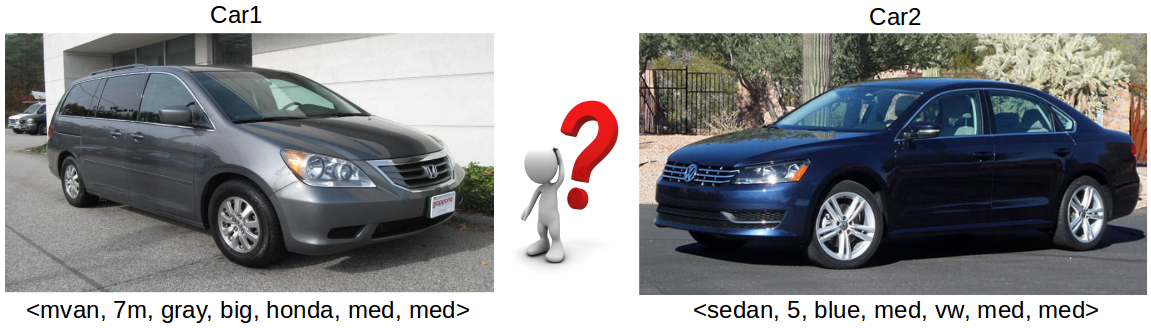
\includegraphics[width=0.95\textwidth]{figs/Cars/individual.png}
	  \caption{Dominance Testing}
	\end{figure}
}

\frameT{Qualitative Preferences}{
	Collective:
	\begin{figure}[ht!]
	  \centering
	    
\includegraphics[width=0.5\textwidth]{figs/Cars/group.png}
	  \caption{Social Choice and Welfare}
	\end{figure}
}
